%%%Variables

%%%
\question When a moving car hits the brakes and comes to rest, its kinetic energy is transferred (through friction with the brake pads) to thermal energy within the brakes\footnote{Some of the kinetic energy is also lost to the road and the air, but ignore that for this problem}. A friend of yours has proposed a design that can extract all of the thermal energy from the brakes and convert it back into kinetic energy when the car accelerates, bringing the car up to the same speed it was before hitting the brakes.

Here's how it works:
\begin{enumerate}
	\item The brake consists of two solid blocks, initially at the same temperature $T_0$. Both blocks have the same heat capacity (call it $C_V$)
	\item When the car brakes, the kinetic energy enters the top block in the form of heat ($Q_{in}$) which raises its temperature (left image)
	\item The temperature difference between the top and bottom block causes heat $Q_h$ to flow out of the top block. The heat flows until both blocks are again at the same temperature. 100\% of this heat is then converted into work, which is able to power the car.
\end{enumerate}
Show your friend that this perpetual motion machine is in fact not possible.
\begin{center}
\begin{tabular}{c|c}
		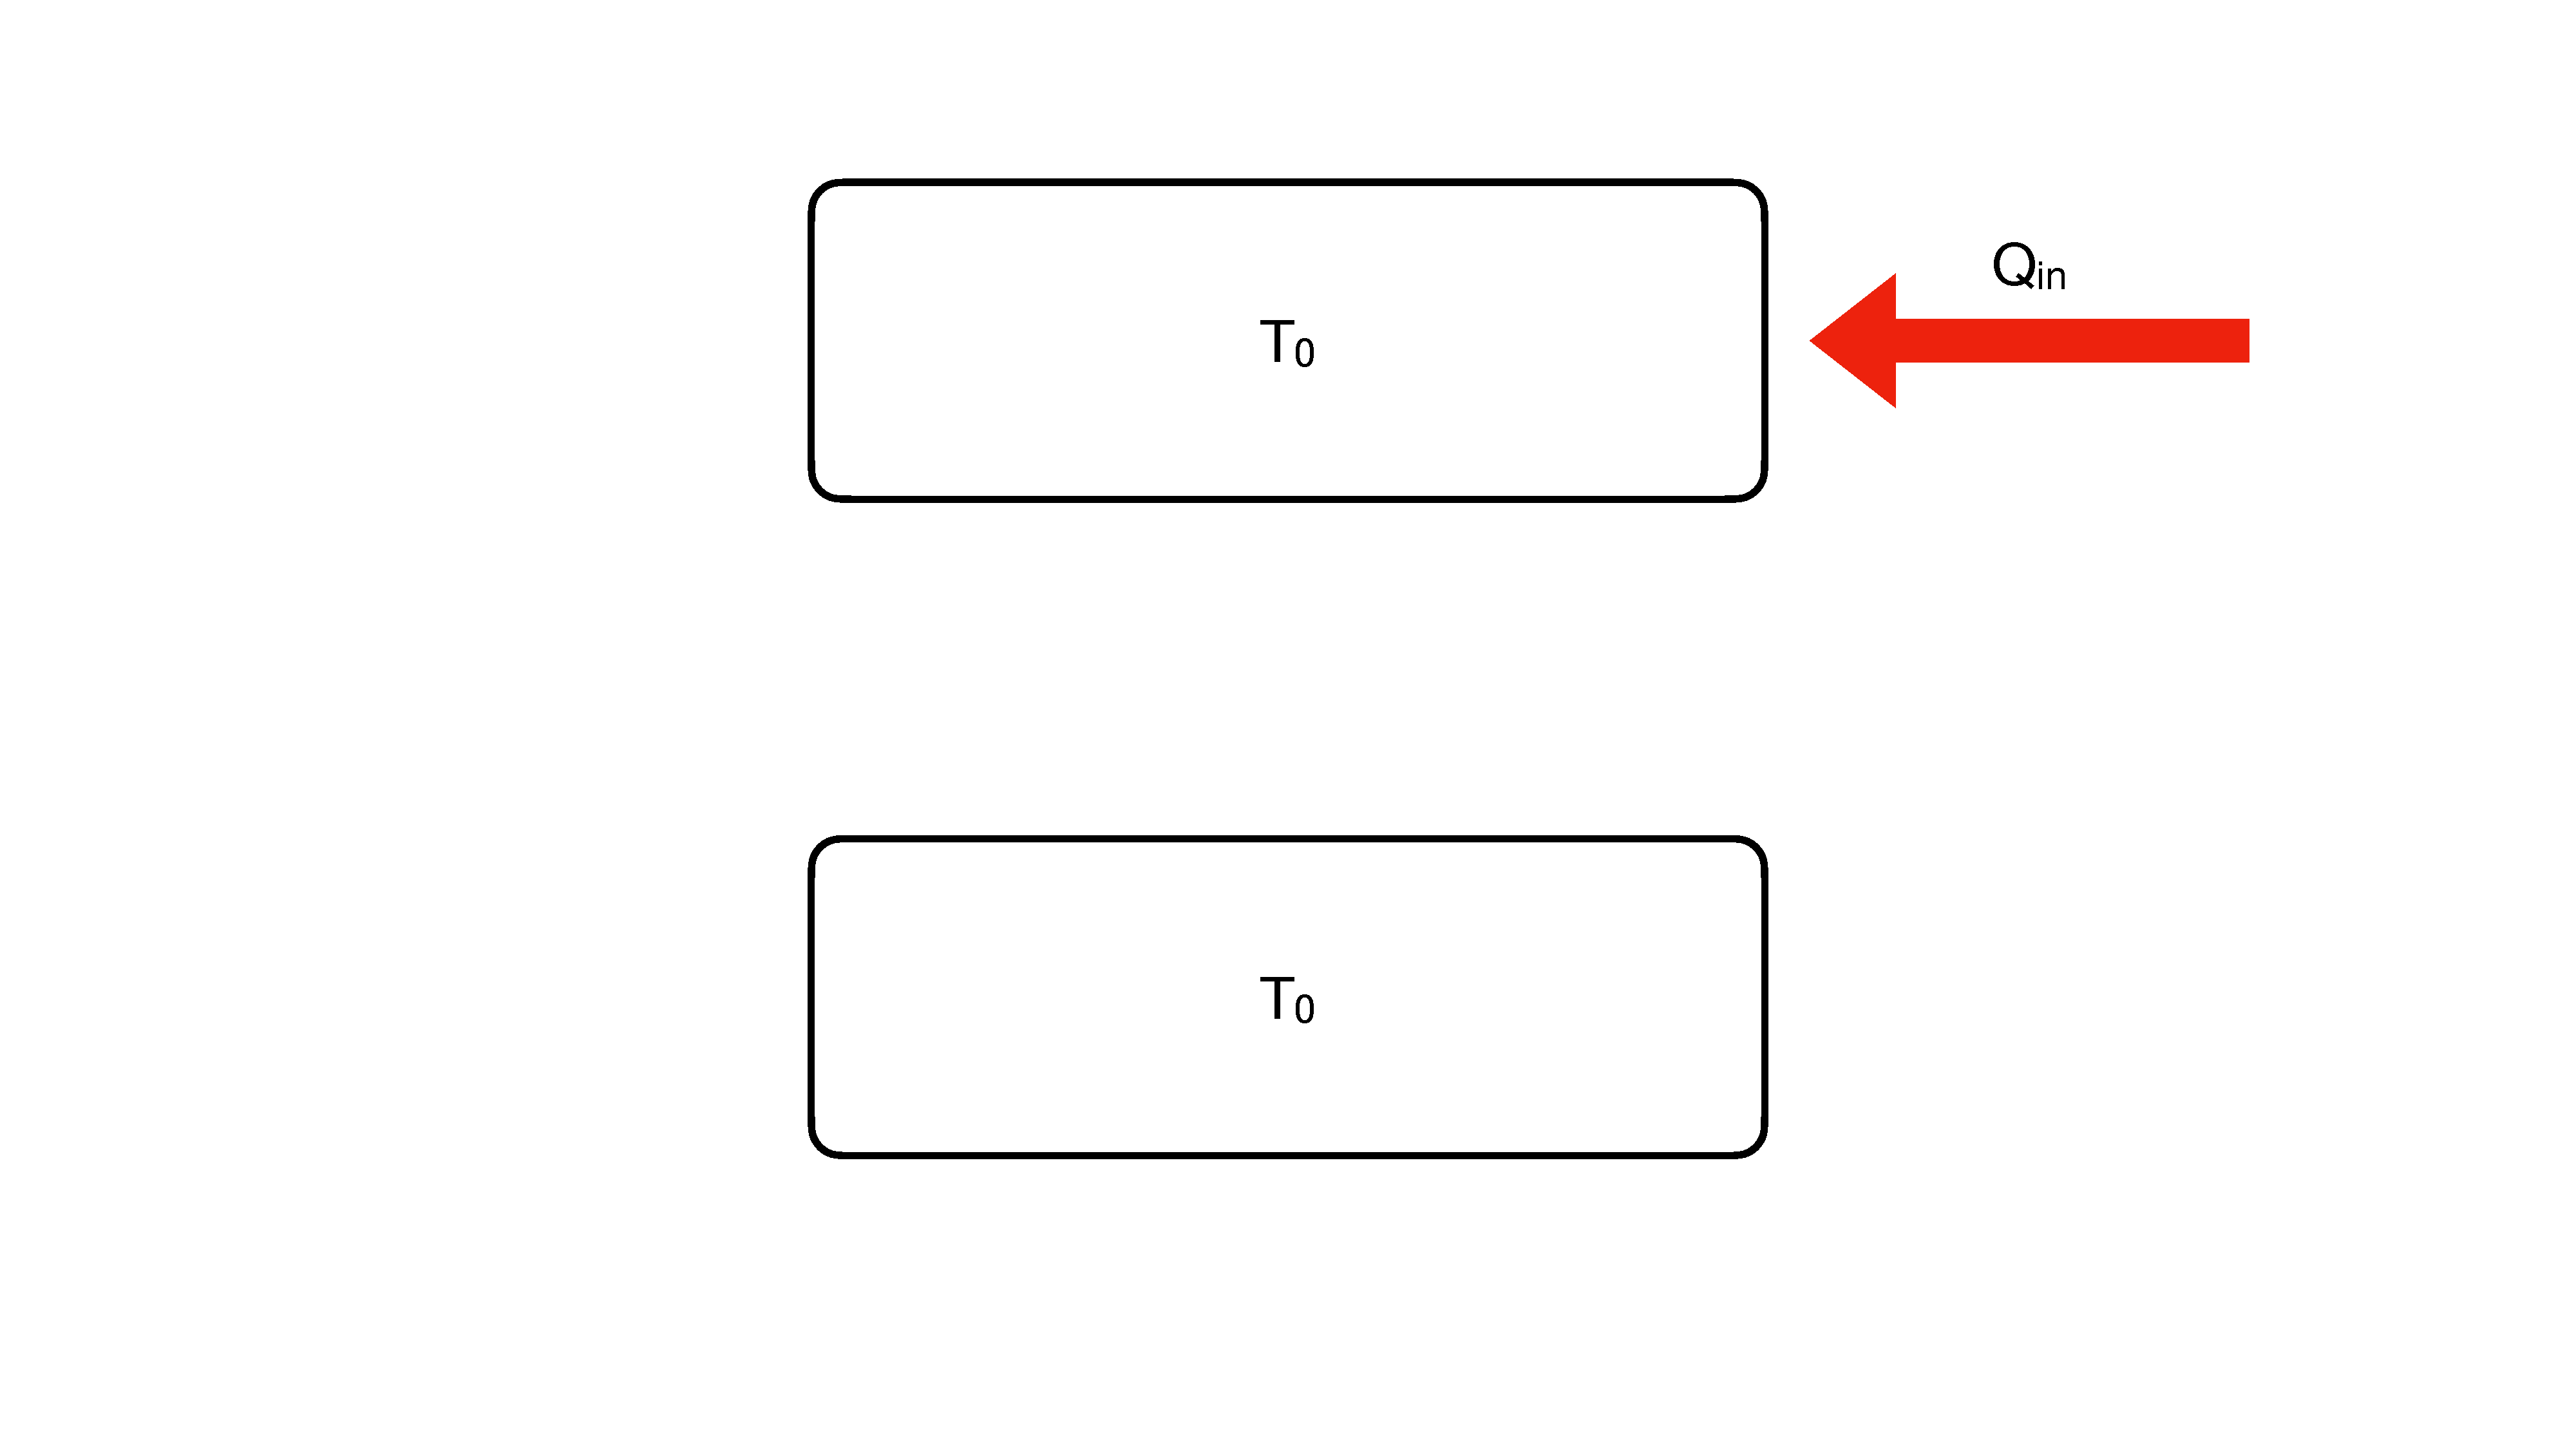
\includegraphics[width=5cm]{heat_bath1.pdf}&	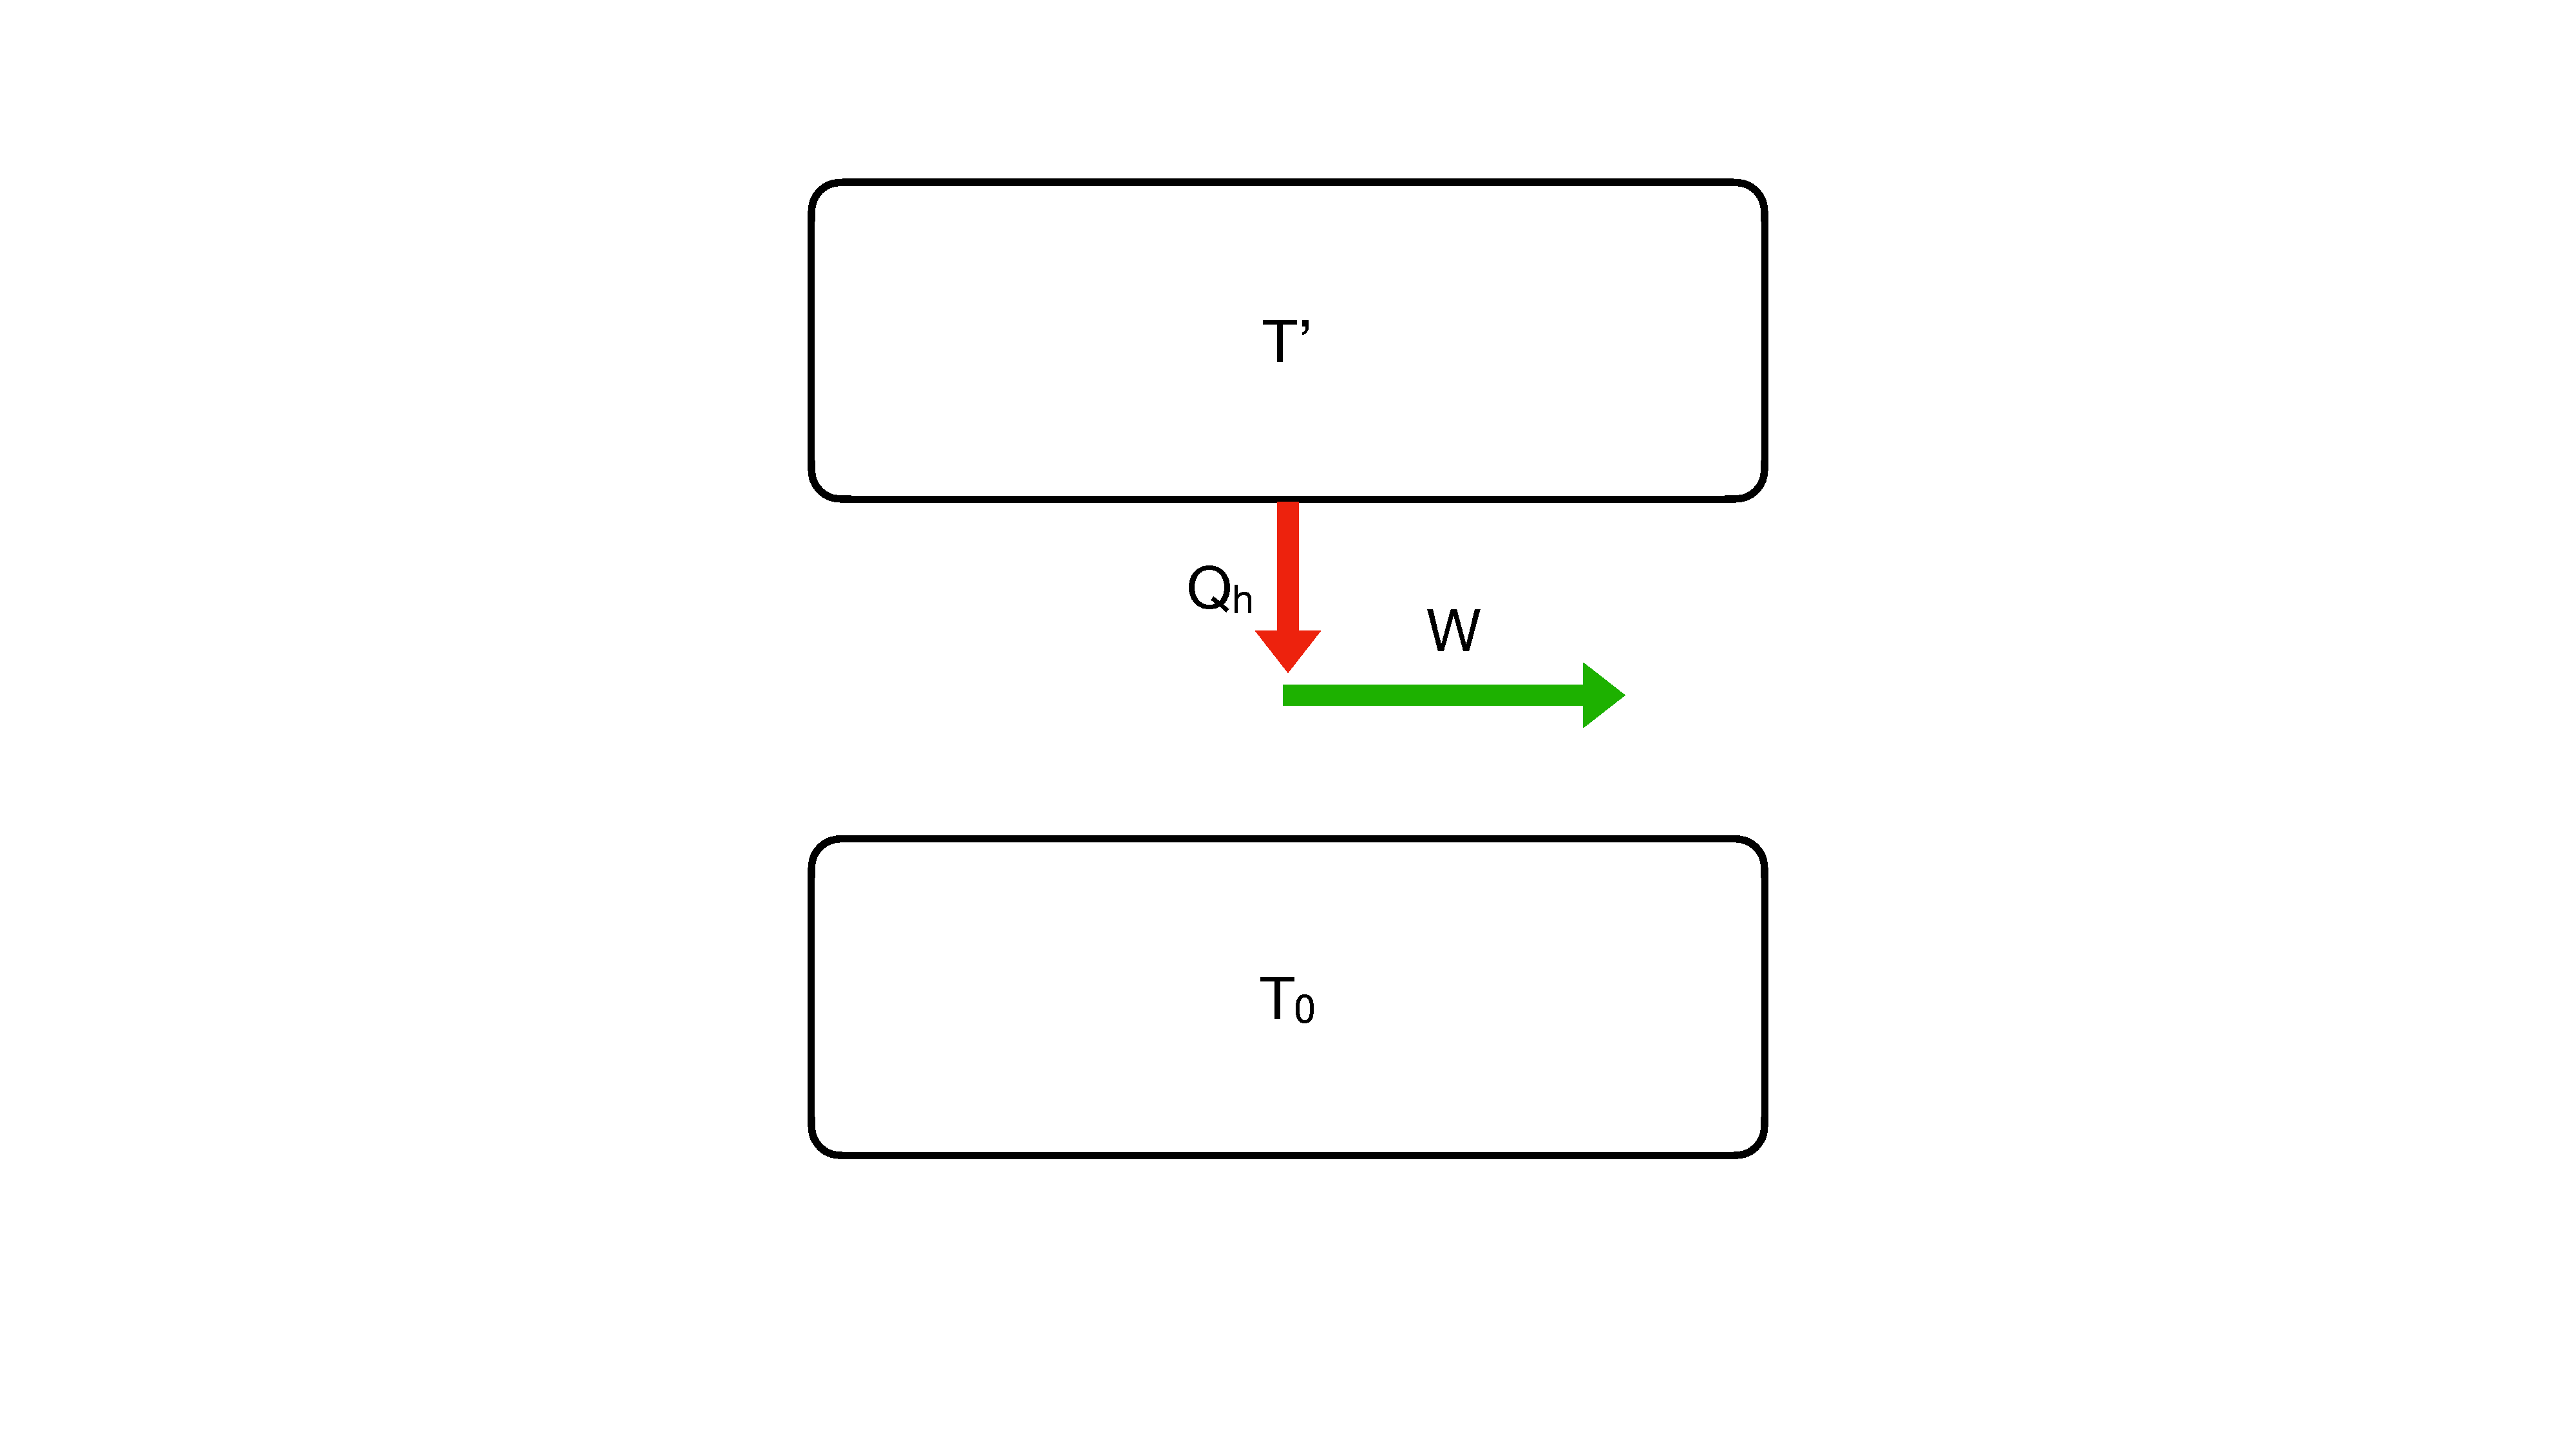
\includegraphics[width=3.5cm]{heat_bath2.pdf}\\
\end{tabular}
\end{center}


\begin{parts}
	\part[5] After an amount of heat $Q_{in}$ enters the top block, what is its new temperature?
	\part[5] What is the change in entropy of the system as depicted in the right panel of the figure ($\Delta S$ of the top block as an amount of heat $Q_h$ leaves the block and the block returns to its original temperature $T_0$.) Explain why this ensures the mechanism shown in the figure is impossible (assuming the work can be done without creating any new entropy).
	\part[10] Assume that instead of all of $Q_h$ being converted into work, some of it is instead converted into ``waste heat'' $Q_c$, which flows into the bottom block and raises its temperature, thus $W=Q_h-Q_c$. This heat continues to flow until the temperatures of the top and bottom block are equal. What is the final temperature of the blocks? Show that if $Q_c>0$, then $Q_h$ must be strictly less than $Q_{in}$.
	
	\part[10] Then show that, in order to satisfy the laws of thermodynamics, $Q_c$ must be greater than 0, hence $W<Q_h<Q_{in}$; i.e., some of the input energy $Q_{in}$ is necessarily ``lost'' and cannot be recovered to power the car.
\end{parts}